\newif\ifsolutions
\solutionstrue % Show solutions
%\solutionsfalse % Hide solutions

\documentclass{article}
\usepackage{geometry}
\geometry{margin=1in}
\usepackage{tikz}
\usepackage{amssymb}

% fleqn allows setting indent of display math
\usepackage[fleqn]{amsmath}
\setlength{\mathindent}{0pt} % Set indent
% Disable equation numbering (https://tex.stackexchange.com/a/360378)
\makeatletter
\renewcommand\tagform@[1]{}
\makeatother

% Allow Unicode (some, e.g., © and £ at least)
% https://tex.stackexchange.com/questions/370278/is-there-any-reason-to-use-inputenc
\usepackage[utf8]{inputenc}

% Hyperlinks
\usepackage{hyperref}
\hypersetup{colorlinks=true, urlcolor=blue, linkcolor=blue}

% Prevent indentation of paragraphs
\setlength\parindent{0pt}
\setlength{\parskip}{\baselineskip}

% Spacing above/below equations
% https://tex.stackexchange.com/a/69678
\AtBeginDocument{%
 \abovedisplayskip=-\parskip
 \abovedisplayshortskip=-\parskip
 \belowdisplayskip=0pt
 \belowdisplayshortskip=0pt
}

% Allow 3 additional subsection levels
% https://tex.stackexchange.com/a/60212
\usepackage{titlesec}
\setcounter{secnumdepth}{6}
% H4 in HTML
\titleformat{\paragraph}{\normalfont\normalsize\bfseries}{\theparagraph}{1em}{}
\titlespacing*{\paragraph}{0pt}{3.25ex plus 1ex minus .2ex}{1.5ex plus .2ex}
% H5 in HTML
\titleformat{\subparagraph}{\normalfont\normalsize\bfseries}{\thesubparagraph}{1em}{}
\titlespacing*{\subparagraph}{0pt}{3.25ex plus 1ex minus .2ex}{1.5ex plus .2ex}
% H6 in HTML
\titleformat{\subsubparagraph}{\normalfont\normalsize\bfseries}{\thesubsubparagraph}{1em}{}
\titlespacing*{\subsubparagraph}{0pt}{3.25ex plus 1ex minus .2ex}{1.5ex plus .2ex}

% So enumerate at all levels is numbers
% https://tex.stackexchange.com/questions/78842/nested-enumeration-numbering
\renewcommand{\labelenumii}{\arabic{enumii}.}
\renewcommand{\labelenumiii}{\arabic{enumiii}.}
\renewcommand{\labelenumiv}{\arabic{enumiv}.}

\renewcommand{\mbox}{\text}
\newcommand{\ds}[0]{\displaystyle}
\newcommand{\ihat}[0]{\hat{\boldsymbol{\imath}}}
\newcommand{\jhat}[0]{\hat{\boldsymbol{\jmath}}}
\newcommand{\khat}[0]{\hat{\boldsymbol{k}}}
\newcommand{\xhat}[0]{\hat{\mathbf{x}}}
\newcommand{\yhat}[0]{\hat{\mathbf{y}}}
\newcommand{\zhat}[0]{\hat{\mathbf{z}}}
\newcommand{\rhat}[0]{\hat{\mathbf{r}}}
\newcommand{\bfvec}[1]{\vec{\mathbf{#1}}}
\newcommand{\bfcdot}[0]{\boldsymbol{\cdot}}

\usepackage{fancyhdr}
\pagestyle{fancy}
\lhead{Kirchhoff's Circuit Laws}
\rhead{\thepage}
\fancyfoot{}

\begin{document}

\section{Introduction}

To find the current through each resistor in a circuit with only resistors and batteries, Kirchhoff's Current Law and Kirchhoff's Voltage Law can be used.

\begin{enumerate}

  \item Kirchhoff's Current Law (KCL): The sum of all currents entering and exiting a junction is zero. Or, equivalently, the current flowing into a junction is equal to the current flowing out of a junction.

  \item Kirchhoff's Voltage Law (KVL): The sum of all voltage changes around a closed loop is zero.

\end{enumerate}

\textbf{General procedure}

To find the values of currents in a circuit, 

\begin{enumerate}

  \item assume directions of current,

  \item write equations for KCL for junctions,

  \item write equations for KVL for loops, and

  \item solve for currents. If you get a negative value for a current, the actual direction of current flow is opposite to what you assumed in 1.

\end{enumerate}

To apply KVL, draw a closed loop and choose a direction to step around the loop. 

\begin{enumerate}

  \item If stepping around the loop requires a step across a battery with emf $\mathcal{E}$ and the $-$ side is encountered first, the voltage change is $+\mathcal{E}$. If the $+$ side is encountered first, the voltage change is $-\mathcal{E}$. \emph{The direction of current through the battery does not matter.}

  \item If stepping around the loop requires a step across a resistor $R$ and the direction of current $I$ through the resistor is the same as the step direction, the voltage change is $-IR$. If the current is opposite the step direction, the voltage change is $+IR$.

\end{enumerate}

A common error is to assume every loop equation requires an emf.

\textbf{Note on Equivalent Resistances}

You may have already had experience solving for currents in circuits using equivalent resistances. In this activity, do not use equivalent resistances unless asked. The motivation is that you will better understand their interpretation and derivation after solving for currents without using equivalent resistances.

\ifsolutions

\else

\newpage
\fi

\section{Single Loop}

Only KVL is needed to find the current in a single-loop circuit.

\begin{enumerate}

  \item The direction of the unknown current $I$ in the following circuit is assumed to be counterclockwise. Write the equation for KVL by stepping around the loop counterclockwise; then solve for $I$ in terms of $\mathcal{E}$ and $R$.

        \input{figures/Single_Loop_CCW.tikz}

        \ifsolutions
        \textbf{Answer:} $\mathcal{E}-IR-IR=0 \quad \Rightarrow \quad I=\mathcal{E}/2R$
        \fi

  \item The direction of current $I$ in the following circuit was assumed to be clockwise. Write the equation for KVL stepping around the loop counterclockwise; then solve for $I$ in terms of $\mathcal{E}$ and $R$.

        \input{figures/Single_Loop_CW.tikz}

        \ifsolutions
        \textbf{Answer:} $\mathcal{E}+IR+IR=0 \quad \Rightarrow \quad I=-\mathcal{E}/2R$
        \fi

  \item Which value for $I$ found above is correct?

        \ifsolutions
        \textbf{Answer}: Both are correct. A negative current is equivalent to a positive current in the opposite direction.
        \else
        \vskip 36pt
        \fi

  \item In part 1., a counterclockwise current was assumed, and you stepped in the counterclockwise direction. If you stepped clockwise, would your answer for $I$ be different?

        \ifsolutions
        \textbf{Answer}: Answer same. KVL is $-\mathcal{E}+IR+IR=0 \quad \Rightarrow \quad I=\mathcal{E}/2R$
        \else
        \vskip 36pt
        \fi

  \item For the first circuit considered above, if you remove the bottom resistor and replace the top resistor with a resistor with resistance $2R$, the following circuit results. What is the current $I$ for this circuit?

        

\tikzset{every picture/.style={line width=0.75pt}} %set default line width to 0.75pt        

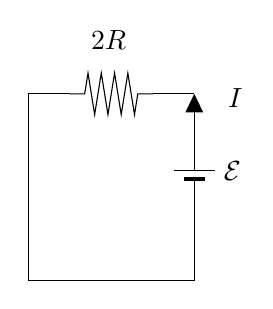
\begin{tikzpicture}[x=0.75pt,y=0.75pt,yscale=-1,xscale=1]
%uncomment if require: \path (0,165); %set diagram left start at 0, and has height of 165

%Shape: Resistor [id:dp642022856937654] 
\draw   (30,40) -- (37.2,40) -- (38.8,30) -- (42,50) -- (45.2,30) -- (48.4,50) -- (51.6,30) -- (54.8,50) -- (58,30) -- (61.2,50) -- (62.8,40) -- (70,40) ;
%Straight Lines [id:da44085423383571] 
\draw    (70,40) -- (90,40) ;
%Straight Lines [id:da8302389383510358] 
\draw    (90,100) -- (90,130) ;
%Straight Lines [id:da2830777981311956] 
\draw    (70,130) -- (90,130) ;
%Straight Lines [id:da2903003917360325] 
\draw    (10,40) -- (30,40) ;
%Straight Lines [id:da5654282060441964] 
\draw    (10,130) -- (70,130) ;
%Straight Lines [id:da4525798154990017] 
\draw    (10,40) -- (10,130) ;
%Straight Lines [id:da23681722570448738] 
\draw    (80,77) -- (100,77) ;
%Straight Lines [id:da2106938932782303] 
\draw [line width=1.5]    (85,81) -- (95,81) ;
%Straight Lines [id:da4202462894704919] 
\draw    (90,81) -- (90,100) ;
%Straight Lines [id:da13525425547720427] 
\draw    (90,43) -- (90,77) ;
\draw [shift={(90,40)}, rotate = 90] [fill={rgb, 255:red, 0; green, 0; blue, 0 }  ][line width=0.08]  [draw opacity=0] (8.93,-4.29) -- (0,0) -- (8.93,4.29) -- cycle    ;

% Text Node
\draw (39,8.4) node [anchor=north west][inner sep=0.75pt]    {$2R$};
% Text Node
\draw (103,71.4) node [anchor=north west][inner sep=0.75pt]    {$\mathcal{E}$};
% Text Node
\draw (105,36.4) node [anchor=north west][inner sep=0.75pt]    {$I$};


\end{tikzpicture}


        \ifsolutions
        \textbf{Answer}: $I=\mathcal{E}/2R$ in counterclockwise direction. The fact that the answer here is the same as in 1. is related to the formula for the equivalent resistance of resistors in series: $R_{\text{eq}}=R_1+R_2$. Two resistors are in series if only one current path exists between them.
        \fi

\end{enumerate}

\ifsolutions

\else

\newpage
\fi

\section{Multiple Loops I}

\input{figures/Parallel.tikz}

\begin{enumerate}

  \item Use KCL at junction $X$ and KVL for loops $A$ and $B$ to show that $I_o=\mathcal{E}\left(\frac{1}{R_1}+\frac{1}{R_2}\right)$.

        \ifsolutions
        \textbf{Answer}:

        KVL for $A$: $+\mathcal{E}-I_1R_1=0\quad\Rightarrow\quad I_1=\mathcal{E}/R_1$

        KVL for $B$: $+I_1R_1-I_2R_2=0 \quad\Rightarrow\quad I_2 = I_1 R_1/R_2 = \mathcal{E}/R_2$

        KCL at $X$: $I_o=I_1+I_2 = \mathcal{E}/R_1 + \mathcal{E}/R_2 = \mathcal{E}\left(\frac{1}{R_1}+\frac{1}{R_2}\right)$
        \else
        \vskip 120pt
        \fi

\end{enumerate}

\begin{enumerate}

  \item[2.] If $R_2 > R_1$, which resistor will have more current?

            \ifsolutions
            \textbf{Answer}:

            $$\frac{I_2}{I_1} = \frac{R_1}{R_2} \quad \Rightarrow \quad I_2 < I_1$$ 

            One can also use the water flow analogy. If $R_2$ resists flow more than $R_1$, there will be more flow through $R_1$.
            \else
            \vskip 60pt
            \fi

  \item[3.] If $R_1 \rightarrow 0$, what happens to $I_o$, $I_1$, and $I_2$?

            \ifsolutions
            \textbf{Answer}: $I_o \rightarrow \infty$, $I_1 \rightarrow \infty$, and $I_2\rightarrow 0$. In this case, we say that resistor $R_2$ is ``shorted" because little current flows through it relative to $R_1$.
            \else

            \newpage
            \fi

\end{enumerate}

%4. Suppose the two resistors were replaced with a resistor with a resistance of $1/\left(\frac{1}{R_1}+\frac{1}{R_2}\right)$ as shown below. What is $I_o$?

\section{Multiple Loops II}

Assume the direction of currents $I_1$, $I_2$, and $I_3$ in the following circuit are as shown.



\tikzset{every picture/.style={line width=0.75pt}} %set default line width to 0.75pt        

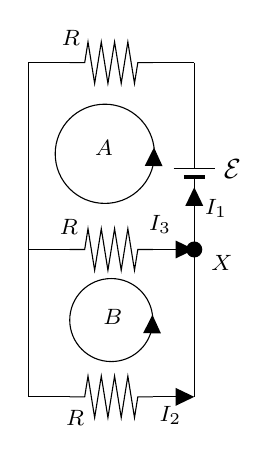
\begin{tikzpicture}[x=0.75pt,y=0.75pt,yscale=-1,xscale=1]
%uncomment if require: \path (0,212); %set diagram left start at 0, and has height of 212

%Shape: Resistor [id:dp4435768995868634] 
\draw   (33,20) -- (40.2,20) -- (41.8,10) -- (45,30) -- (48.2,10) -- (51.4,30) -- (54.6,10) -- (57.8,30) -- (61,10) -- (64.2,30) -- (65.8,20) -- (73,20) ;
%Straight Lines [id:da6348738339014448] 
\draw    (73,20) -- (93,20) ;
%Straight Lines [id:da5094119689345933] 
\draw    (93,20) -- (93,40) ;
%Straight Lines [id:da29132347297122374] 
\draw    (93,83) -- (93,110) ;
\draw [shift={(93,80)}, rotate = 90] [fill={rgb, 255:red, 0; green, 0; blue, 0 }  ][line width=0.08]  [draw opacity=0] (8.93,-4.29) -- (0,0) -- (8.93,4.29) -- cycle    ;
%Shape: Resistor [id:dp4960144413750487] 
\draw   (33,110) -- (40.2,110) -- (41.8,100) -- (45,120) -- (48.2,100) -- (51.4,120) -- (54.6,100) -- (57.8,120) -- (61,100) -- (64.2,120) -- (65.8,110) -- (73,110) ;
%Straight Lines [id:da24469614531440342] 
\draw    (73,110) -- (90,110) ;
\draw [shift={(93,110)}, rotate = 180] [fill={rgb, 255:red, 0; green, 0; blue, 0 }  ][line width=0.08]  [draw opacity=0] (8.93,-4.29) -- (0,0) -- (8.93,4.29) -- cycle    ;
%Straight Lines [id:da22765892469283] 
\draw    (13,20) -- (33,20) ;
%Straight Lines [id:da17732812907855178] 
\draw    (13,110) -- (33,110) ;
%Straight Lines [id:da9666768486239514] 
\draw    (13,20) -- (13,110) ;
%Shape: Resistor [id:dp6772651137474663] 
\draw   (33,181) -- (40.2,181) -- (41.8,171) -- (45,191) -- (48.2,171) -- (51.4,191) -- (54.6,171) -- (57.8,191) -- (61,171) -- (64.2,191) -- (65.8,181) -- (73,181) ;
%Straight Lines [id:da9288559665794871] 
\draw    (13,110) -- (13,181) ;
%Straight Lines [id:da06047002217821351] 
\draw    (93,110) -- (93,181) ;
\draw [shift={(93,110)}, rotate = 90] [color={rgb, 255:red, 0; green, 0; blue, 0 }  ][fill={rgb, 255:red, 0; green, 0; blue, 0 }  ][line width=0.75]      (0, 0) circle [x radius= 3.35, y radius= 3.35]   ;
%Straight Lines [id:da0286509869159568] 
\draw    (73,181) -- (90,181) ;
\draw [shift={(93,181)}, rotate = 180] [fill={rgb, 255:red, 0; green, 0; blue, 0 }  ][line width=0.08]  [draw opacity=0] (8.93,-4.29) -- (0,0) -- (8.93,4.29) -- cycle    ;
%Straight Lines [id:da6480632637542392] 
\draw    (13,181) -- (33,181) ;
%Shape: Arc [id:dp3431106756408584] 
\draw  [draw opacity=0] (73.47,67.89) .. controls (71.57,79.19) and (61.74,87.8) .. (49.9,87.8) .. controls (36.7,87.8) and (26,77.1) .. (26,63.9) .. controls (26,50.7) and (36.7,40) .. (49.9,40) .. controls (62.73,40) and (73.21,50.12) .. (73.78,62.81) -- (49.9,63.9) -- cycle ; \draw   (73.47,67.89) .. controls (71.57,79.19) and (61.74,87.8) .. (49.9,87.8) .. controls (36.7,87.8) and (26,77.1) .. (26,63.9) .. controls (26,50.7) and (36.7,40) .. (49.9,40) .. controls (62.73,40) and (73.21,50.12) .. (73.78,62.81) ;  
%Straight Lines [id:da24655244368311546] 
\draw    (73.47,67.89) -- (73.55,63.85) ;
\draw [shift={(73.61,60.85)}, rotate = 91.13] [fill={rgb, 255:red, 0; green, 0; blue, 0 }  ][line width=0.08]  [draw opacity=0] (8.93,-4.29) -- (0,0) -- (8.93,4.29) -- cycle    ;
%Shape: Arc [id:dp8851152110706482] 
\draw  [draw opacity=0] (72.72,147.34) .. controls (71.14,156.79) and (62.91,164) .. (53,164) .. controls (41.95,164) and (33,155.05) .. (33,144) .. controls (33,132.95) and (41.95,124) .. (53,124) .. controls (63.74,124) and (72.5,132.46) .. (72.98,143.09) -- (53,144) -- cycle ; \draw   (72.72,147.34) .. controls (71.14,156.79) and (62.91,164) .. (53,164) .. controls (41.95,164) and (33,155.05) .. (33,144) .. controls (33,132.95) and (41.95,124) .. (53,124) .. controls (63.74,124) and (72.5,132.46) .. (72.98,143.09) ;  
%Straight Lines [id:da6299489125610516] 
\draw    (72.72,147.34) -- (72.78,144.45) ;
\draw [shift={(72.84,141.45)}, rotate = 91.13] [fill={rgb, 255:red, 0; green, 0; blue, 0 }  ][line width=0.08]  [draw opacity=0] (8.93,-4.29) -- (0,0) -- (8.93,4.29) -- cycle    ;
%Straight Lines [id:da035127828787047566] 
\draw    (93,34) -- (93,71) ;
%Straight Lines [id:da06981066985977469] 
\draw    (83,71) -- (103,71) ;
%Straight Lines [id:da07498872749287244] 
\draw [line width=1.5]    (88,75) -- (98,75) ;
%Straight Lines [id:da9169274458375447] 
\draw    (93,75) -- (93,94) ;

% Text Node
\draw (27,94.4) node [anchor=north west][inner sep=0.75pt]  [font=\footnotesize]  {$R$};
% Text Node
\draw (97,84.4) node [anchor=north west][inner sep=0.75pt]  [font=\footnotesize]  {$I_{1}$};
% Text Node
\draw (75,184.4) node [anchor=north west][inner sep=0.75pt]  [font=\footnotesize]  {$I_{2}$};
% Text Node
\draw (70,92.4) node [anchor=north west][inner sep=0.75pt]  [font=\footnotesize]  {$I_{3}$};
% Text Node
\draw (100,111.4) node [anchor=north west][inner sep=0.75pt]  [font=\footnotesize]  {$X$};
% Text Node
\draw (44,56.4) node [anchor=north west][inner sep=0.75pt]  [font=\footnotesize]  {$A$};
% Text Node
\draw (30,186.4) node [anchor=north west][inner sep=0.75pt]  [font=\footnotesize]  {$R$};
% Text Node
\draw (28,3.4) node [anchor=north west][inner sep=0.75pt]  [font=\footnotesize]  {$R$};
% Text Node
\draw (48,137.4) node [anchor=north west][inner sep=0.75pt]  [font=\footnotesize]  {$B$};
% Text Node
\draw (106,65.4) node [anchor=north west][inner sep=0.75pt]    {$\mathcal{E}$};


\end{tikzpicture}


\begin{enumerate}

  \item Write the equation for KVL for loop $A$.

        \ifsolutions
        \textbf{Answer}: $+\mathcal{E}-I_1R-I_3R=0$
        \else
        \vskip 36pt
        \fi

  \item Write the equation for KVL for loop $B$.

        \ifsolutions
        \textbf{Answer}: $I_3R-I_2R=0$. A common error is to attempt to include $\mathcal{E}$ in this equation. When using KVL, the only elements that appear in the equation are elements that are stepped across when going around the chosen loop.
        \else
        \vskip 36pt
        \fi

  \item Write the equation for KCL for junction X.

        \ifsolutions
        \textbf{Answer}: $I_3+I_2=I_1$
        \else
        \vskip 36pt
        \fi

  \item Use the three equations found above to solve for the three unknowns, $I_1$, $I_2$, and $I_3$ in terms of $\mathcal{E}$ and $R$.

        \ifsolutions
        \textbf{Answer}:

        Eqn 1: $+\mathcal{E}-I_1R-I_3R=0$

        Eqn 2: $I_3R-I_2R=0$

        Eqn 3: $I_3+I_2=I_1$

        From Eqn 2., $I_2=I_3$ (this is expected, why?). Sub this into Eqn. 3 to get $I_3=I_1/2$. Plug this into Eqn 1. to get $I_1=(2/3)(\mathcal{E}/R)$. Additional substitution gives $I_2=I_3=(1/3)(\mathcal{E}/R)$.
        \else
        \vskip 96pt
        \fi

  \item Check your answers by plugging your values for $I_1$, $I_2$, and $I_3$ into the equations that you wrote for parts 1.-3.

        \ifsolutions
        \textbf{Comment}: This is an important step. Sign errors in KVL and KCL are common, as are algebraic errors, and this check will determine if you made an error.
        \else

        \newpage
        \fi

\end{enumerate}

\section{Multiple Loops II}

In the circuit for the previous problem, there are three possible loops. The third loop is loop $C$, which is indicated below.



\tikzset{every picture/.style={line width=0.75pt}} %set default line width to 0.75pt        

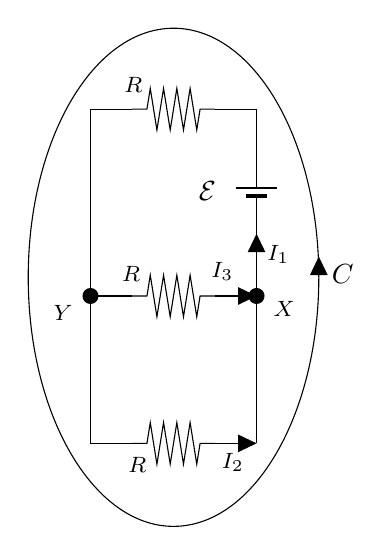
\begin{tikzpicture}[x=0.75pt,y=0.75pt,yscale=-1,xscale=1]
%uncomment if require: \path (0,264); %set diagram left start at 0, and has height of 264

%Shape: Resistor [id:dp17060205471087664] 
\draw   (60,49) -- (67.2,49) -- (68.8,39) -- (72,59) -- (75.2,39) -- (78.4,59) -- (81.6,39) -- (84.8,59) -- (88,39) -- (91.2,59) -- (92.8,49) -- (100,49) ;
%Straight Lines [id:da026559281912648114] 
\draw    (100,49) -- (120,49) ;
%Straight Lines [id:da7617206491414388] 
\draw    (120,49) -- (120,69) ;
%Straight Lines [id:da970382599927843] 
\draw    (120,112) -- (120,139) ;
\draw [shift={(120,109)}, rotate = 90] [fill={rgb, 255:red, 0; green, 0; blue, 0 }  ][line width=0.08]  [draw opacity=0] (8.93,-4.29) -- (0,0) -- (8.93,4.29) -- cycle    ;
%Shape: Resistor [id:dp606783941498729] 
\draw   (60,139) -- (67.2,139) -- (68.8,129) -- (72,149) -- (75.2,129) -- (78.4,149) -- (81.6,129) -- (84.8,149) -- (88,129) -- (91.2,149) -- (92.8,139) -- (100,139) ;
%Straight Lines [id:da17314151648314247] 
\draw    (100,139) -- (117,139) ;
\draw [shift={(120,139)}, rotate = 180] [fill={rgb, 255:red, 0; green, 0; blue, 0 }  ][line width=0.08]  [draw opacity=0] (8.93,-4.29) -- (0,0) -- (8.93,4.29) -- cycle    ;
%Straight Lines [id:da8025234315851337] 
\draw    (40,49) -- (60,49) ;
%Straight Lines [id:da17836496817482805] 
\draw    (40,139) -- (60,139) ;
%Straight Lines [id:da7781781144106024] 
\draw    (40,49) -- (40,139) ;
%Shape: Resistor [id:dp2826362414149479] 
\draw   (60,210) -- (67.2,210) -- (68.8,200) -- (72,220) -- (75.2,200) -- (78.4,220) -- (81.6,200) -- (84.8,220) -- (88,200) -- (91.2,220) -- (92.8,210) -- (100,210) ;
%Straight Lines [id:da8251219225767277] 
\draw    (120,139) -- (120,210) ;
\draw [shift={(120,139)}, rotate = 90] [color={rgb, 255:red, 0; green, 0; blue, 0 }  ][fill={rgb, 255:red, 0; green, 0; blue, 0 }  ][line width=0.75]      (0, 0) circle [x radius= 3.35, y radius= 3.35]   ;
%Straight Lines [id:da4634026204005979] 
\draw    (100,210) -- (117,210) ;
\draw [shift={(120,210)}, rotate = 180] [fill={rgb, 255:red, 0; green, 0; blue, 0 }  ][line width=0.08]  [draw opacity=0] (8.93,-4.29) -- (0,0) -- (8.93,4.29) -- cycle    ;
%Straight Lines [id:da022515967651009827] 
\draw    (40,210) -- (60,210) ;
%Shape: Ellipse [id:dp5645644533895287] 
\draw   (10,130) .. controls (10,63.73) and (41.34,10) .. (80,10) .. controls (118.66,10) and (150,63.73) .. (150,130) .. controls (150,196.27) and (118.66,250) .. (80,250) .. controls (41.34,250) and (10,196.27) .. (10,130) -- cycle ;
%Straight Lines [id:da018587299401993995] 
\draw    (150,130) -- (150,123) ;
\draw [shift={(150,120)}, rotate = 90] [fill={rgb, 255:red, 0; green, 0; blue, 0 }  ][line width=0.08]  [draw opacity=0] (8.93,-4.29) -- (0,0) -- (8.93,4.29) -- cycle    ;
%Straight Lines [id:da8059012117058191] 
\draw    (40,139) -- (40,210) ;
\draw [shift={(40,139)}, rotate = 90] [color={rgb, 255:red, 0; green, 0; blue, 0 }  ][fill={rgb, 255:red, 0; green, 0; blue, 0 }  ][line width=0.75]      (0, 0) circle [x radius= 3.35, y radius= 3.35]   ;
%Straight Lines [id:da9608319101186609] 
\draw    (120,50) -- (120,87) ;
%Straight Lines [id:da022039084729565506] 
\draw    (110,87) -- (130,87) ;
%Straight Lines [id:da0036845135841885313] 
\draw [line width=1.5]    (115,91) -- (125,91) ;
%Straight Lines [id:da22758616610747429] 
\draw    (120,91) -- (120,110) ;

% Text Node
\draw (54,123.4) node [anchor=north west][inner sep=0.75pt]  [font=\footnotesize]  {$R$};
% Text Node
\draw (124,113.4) node [anchor=north west][inner sep=0.75pt]  [font=\footnotesize]  {$I_{1}$};
% Text Node
\draw (102,213.4) node [anchor=north west][inner sep=0.75pt]  [font=\footnotesize]  {$I_{2}$};
% Text Node
\draw (97,121.4) node [anchor=north west][inner sep=0.75pt]  [font=\footnotesize]  {$I_{3}$};
% Text Node
\draw (127,140.4) node [anchor=north west][inner sep=0.75pt]  [font=\footnotesize]  {$X$};
% Text Node
\draw (57,215.4) node [anchor=north west][inner sep=0.75pt]  [font=\footnotesize]  {$R$};
% Text Node
\draw (55,32.4) node [anchor=north west][inner sep=0.75pt]  [font=\footnotesize]  {$R$};
% Text Node
\draw (155,122.4) node [anchor=north west][inner sep=0.75pt]    {$C$};
% Text Node
\draw (21,142.4) node [anchor=north west][inner sep=0.75pt]  [font=\footnotesize]  {$Y$};
% Text Node
\draw (91,82.4) node [anchor=north west][inner sep=0.75pt]    {$\mathcal{E}$};


\end{tikzpicture}


\begin{enumerate}

  \item Write the equation for KVL for loop $C$.

        \ifsolutions
        \textbf{Answer}: $\mathcal{E}-I_1R-I_2R=0$
        \else
        \vskip 36pt
        \fi

  \item Use the equation for KVL for loop $B$ and the KCL equation for junction $X$ along with the KVL equation for loop $C$ to find $I_1$, $I_2$, and $I_3$ in terms of $\mathcal{E}$ and $R$. (You should get the same answers as the previous problem.)

\end{enumerate}

\ifsolutions

\else

\newpage
\fi

\section{Redundant Equations}

When solving circuit problems with multiple loops, you will generally find that you can use KVL and KCL to write more equations than there are unknowns. If you attempt to solve a problem with $N$ unknowns by writing $N$ equations based on KVL and KCL but cannot solve for the unknowns, the reason is that two or more of the equations that you wrote were not independent. To demonstrate this, for the following circuit,



\tikzset{every picture/.style={line width=0.75pt}} %set default line width to 0.75pt        

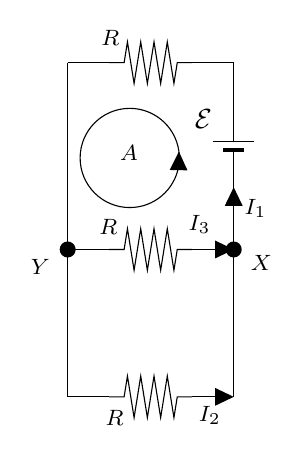
\begin{tikzpicture}[x=0.75pt,y=0.75pt,yscale=-1,xscale=1]
%uncomment if require: \path (0,264); %set diagram left start at 0, and has height of 264

%Shape: Resistor [id:dp2524184722994143] 
\draw   (60,49) -- (67.2,49) -- (68.8,39) -- (72,59) -- (75.2,39) -- (78.4,59) -- (81.6,39) -- (84.8,59) -- (88,39) -- (91.2,59) -- (92.8,49) -- (100,49) ;
%Straight Lines [id:da9831394926513701] 
\draw    (100,49) -- (120,49) ;
%Straight Lines [id:da06903668242243843] 
\draw    (120,49) -- (120,69) ;
%Straight Lines [id:da651338255376767] 
\draw    (120,112) -- (120,139) ;
\draw [shift={(120,109)}, rotate = 90] [fill={rgb, 255:red, 0; green, 0; blue, 0 }  ][line width=0.08]  [draw opacity=0] (8.93,-4.29) -- (0,0) -- (8.93,4.29) -- cycle    ;
%Shape: Resistor [id:dp21864265246191938] 
\draw   (60,139) -- (67.2,139) -- (68.8,129) -- (72,149) -- (75.2,129) -- (78.4,149) -- (81.6,129) -- (84.8,149) -- (88,129) -- (91.2,149) -- (92.8,139) -- (100,139) ;
%Straight Lines [id:da7200722885610089] 
\draw    (100,139) -- (117,139) ;
\draw [shift={(120,139)}, rotate = 180] [fill={rgb, 255:red, 0; green, 0; blue, 0 }  ][line width=0.08]  [draw opacity=0] (8.93,-4.29) -- (0,0) -- (8.93,4.29) -- cycle    ;
%Straight Lines [id:da027217809739622956] 
\draw    (40,49) -- (60,49) ;
%Straight Lines [id:da09434993868871788] 
\draw    (40,139) -- (60,139) ;
%Straight Lines [id:da8448787660328827] 
\draw    (40,49) -- (40,139) ;
%Shape: Resistor [id:dp8794406807534081] 
\draw   (60,210) -- (67.2,210) -- (68.8,200) -- (72,220) -- (75.2,200) -- (78.4,220) -- (81.6,200) -- (84.8,220) -- (88,200) -- (91.2,220) -- (92.8,210) -- (100,210) ;
%Straight Lines [id:da6933787506634865] 
\draw    (120,139) -- (120,210) ;
\draw [shift={(120,139)}, rotate = 90] [color={rgb, 255:red, 0; green, 0; blue, 0 }  ][fill={rgb, 255:red, 0; green, 0; blue, 0 }  ][line width=0.75]      (0, 0) circle [x radius= 3.35, y radius= 3.35]   ;
%Straight Lines [id:da2416286978278488] 
\draw    (100,210) -- (117,210) ;
\draw [shift={(120,210)}, rotate = 180] [fill={rgb, 255:red, 0; green, 0; blue, 0 }  ][line width=0.08]  [draw opacity=0] (8.93,-4.29) -- (0,0) -- (8.93,4.29) -- cycle    ;
%Straight Lines [id:da5424323112360687] 
\draw    (40,210) -- (60,210) ;
%Straight Lines [id:da30984975132395776] 
\draw    (40,139) -- (40,210) ;
\draw [shift={(40,139)}, rotate = 90] [color={rgb, 255:red, 0; green, 0; blue, 0 }  ][fill={rgb, 255:red, 0; green, 0; blue, 0 }  ][line width=0.75]      (0, 0) circle [x radius= 3.35, y radius= 3.35]   ;
%Straight Lines [id:da3059667385706837] 
\draw    (120,50) -- (120,87) ;
%Straight Lines [id:da9581315462885218] 
\draw    (110,87) -- (130,87) ;
%Straight Lines [id:da8139657282656465] 
\draw [line width=1.5]    (115,91) -- (125,91) ;
%Straight Lines [id:da157510882932268] 
\draw    (120,91) -- (120,110) ;
%Shape: Arc [id:dp8118670491021451] 
\draw  [draw opacity=0] (93.47,98.89) .. controls (91.57,110.19) and (81.74,118.8) .. (69.9,118.8) .. controls (56.7,118.8) and (46,108.1) .. (46,94.9) .. controls (46,81.7) and (56.7,71) .. (69.9,71) .. controls (82.73,71) and (93.21,81.12) .. (93.78,93.81) -- (69.9,94.9) -- cycle ; \draw   (93.47,98.89) .. controls (91.57,110.19) and (81.74,118.8) .. (69.9,118.8) .. controls (56.7,118.8) and (46,108.1) .. (46,94.9) .. controls (46,81.7) and (56.7,71) .. (69.9,71) .. controls (82.73,71) and (93.21,81.12) .. (93.78,93.81) ;  
%Straight Lines [id:da2659103659426487] 
\draw    (93.47,98.89) -- (93.55,94.85) ;
\draw [shift={(93.61,91.85)}, rotate = 91.13] [fill={rgb, 255:red, 0; green, 0; blue, 0 }  ][line width=0.08]  [draw opacity=0] (8.93,-4.29) -- (0,0) -- (8.93,4.29) -- cycle    ;

% Text Node
\draw (54,123.4) node [anchor=north west][inner sep=0.75pt]  [font=\footnotesize]  {$R$};
% Text Node
\draw (124,113.4) node [anchor=north west][inner sep=0.75pt]  [font=\footnotesize]  {$I_{1}$};
% Text Node
\draw (102,213.4) node [anchor=north west][inner sep=0.75pt]  [font=\footnotesize]  {$I_{2}$};
% Text Node
\draw (97,121.4) node [anchor=north west][inner sep=0.75pt]  [font=\footnotesize]  {$I_{3}$};
% Text Node
\draw (127,140.4) node [anchor=north west][inner sep=0.75pt]  [font=\footnotesize]  {$X$};
% Text Node
\draw (57,215.4) node [anchor=north west][inner sep=0.75pt]  [font=\footnotesize]  {$R$};
% Text Node
\draw (55,32.4) node [anchor=north west][inner sep=0.75pt]  [font=\footnotesize]  {$R$};
% Text Node
\draw (21,142.4) node [anchor=north west][inner sep=0.75pt]  [font=\footnotesize]  {$Y$};
% Text Node
\draw (100,70.4) node [anchor=north west][inner sep=0.75pt]    {$\mathcal{E}$};
% Text Node
\draw (64,87.4) node [anchor=north west][inner sep=0.75pt]  [font=\footnotesize]  {$A$};


\end{tikzpicture}


\begin{enumerate}

  \item write the KCL equation for junction X,

        \ifsolutions
        \textbf{Answer}: $-I_1+I_2+I_3$
        \else
        \vskip 36pt
        \fi

  \item write the KCL equation for junction Y,

        \ifsolutions
        \textbf{Answer}: $+I_1-I_2-I_3=0$
        \else
        \vskip 36pt
        \fi

  \item write the KVL equation for loop $A$, and

        \ifsolutions
        \textbf{Answer}: $+\mathcal{E}-I_1R-I_3R=0$
        \else
        \vskip 36pt
        \fi

  \item Is it possible to use the above three equations to solve for $I_1$, $I_2$, and $I_3$ in terms of $\mathcal{E}$ and $R$? If yes, do it. If no, explain why.

        \ifsolutions
        \textbf{Answer}: No. The equation for junction $X$ can be turned into the equation for junction $Y$ by multiplying all terms in either equation by $-1$. Thus, the equations are not independent. Given that three independent equations are needed to solve for three unknowns, a solution is impossible with the equations requested in parts 1.--3.
        \fi

\end{enumerate}

\end{document}